% This document is available under the GNU Free Documentation License
% Copyright (C) 2011 --- Benjamin Woodruff
% See the file LICENSE for copying conditions.

\documentclass[letterpaper, 12pt]{article}

\usepackage[in]{fullpage}
\usepackage{multicol}
\usepackage{mdwlist}
\usepackage{hyperref}
\usepackage{graphicx}
\usepackage[american]{babel} 
\usepackage{biblatex}

\pagestyle{empty}
\defbibheading{blank}{}

\addbibresource{citations.bib}

\begin{document}

\begin{flushleft}
Path-finding with Dijkstra's Algorithm\\
Benjamin Woodruff\\
\href{mailto:odetopi.e@gmail.com}{odetopi.e@gmail.com},
Duncan U.~Fletcher High School
\end{flushleft}

\vspace{0.25in}

\begin{huge}
    \begin{center}
        \textbf{Path-finding with Dijkstra's Algorithm}
    \end{center}
\end{huge}
\vspace{.5in}

\begin{multicols}{2}

\section{Abstract}

As we develop and advance in the Botball competition, the need arises to build
more and more intelligent systems. Path-finding isn't only about reducing the
repetitive work on programmers, but also allowing robots to make decisions on
the fly. As an alternative to techniques such as line-following, or as an aid,
path-finding can take advantage of the largely static Botball board layout. This
paper seeks to describe a technique and example implementation by which a
perfectly optimal, non-intersecting, easily navigable path can be found. In
addition, this document outlines surrounding support systems for working with
such paths, and putting things into practice.

\section{Reasoning}

\subsection{An Example Problem}

Imagine you have a movement library, such as CBCJVM's \cite{cbcjvm2010}, that
allows for simple geometric movements and position tracking \footnote{With the
right calculations, as long as all your motions happen through a single movement
library, you should be able to dynamically determine exactly where you are at
any point in time}. The robot successfully finds a set of blocks with it's
camera, but now you have to figure out how to navigate back to your drop-off
point. There's a few simple answers, such as reversing the movements that you
took to get the blocks, returning you to a known point, but all of these are
inefficient. If you try to simply move from one point to another, using position
tracking, you have no easy way of handling if there is an object in the way of
your path.

\subsection{How Pathfinding can Help}

A proper path-finding system already knows the layout of obstacles on the board,
either through static (programmer) input, or through dynamically (sensor)
inputted information. With this, the system should be able to determine the best
way to get from Point A to Point B, avoiding everything else
in-between \cite{wikipathfinding}. This can then be distilled into a simple set
of actions, such as

\begin{enumerate*}
    \item Rotate 37 degrees clockwise
    \item Move 36 cm forward
    \item Rotate 84 degrees counter-clockwise
    \item Move 15 cm forward
\end{enumerate*}

\section{A* (A-Star)}

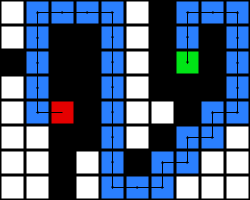
\includegraphics[width=\columnwidth]{img/a_star.pdf}

The typical way of solving such a problem, as has been done by teams such as
Norman High School in the past, has been to turn the board into a grid, and to
utilize the simple A* algorithm to then generate a path on the grid. Such a path
is then traced and turned into a set of movements, like above. Unfortunately a
specific description of the algorithm is beyond the scope of this document, but
there is a plethora of places, online and otherwise, to find such a description.
\cite{wikiastar}

However, such a system works in a non-optimal manner. Our robots do not operate
on a grid, and, as a result, the generated paths can end up including far more
points than ideal. Additionally, the A* algorithm does not guarantee that the
resultant path, even in a grid setting, is the shortest one.

While this is an interesting system to work with, and an even more interesting
proof of concept, the more geometrically aligned Dijkstra's algorithm appears a
better choice.

\section{Graph Theory}

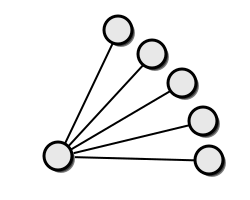
\includegraphics[width=\columnwidth]{img/graph_theory.pdf}

Let's start by turning the board into the simplest representation we can: a set
of line segments. Each of these line segments have two end-points, or nodes, and
a group of lines, sharing nodes at vertices form polygons. The board can be
represented through a set of inaccessible polygon areas, and otherwise open
area.

When you are forming an optimal path, assuming the robot itself is a point-mass,
the only nodes included in the path will be the starting point, the ending
point, and the vertices of the polygons on the map. This assumption greatly
reduces our search-space.

\subsection{Line-of-Sight}

As obvious as it seems to us that the robot cannot simply pass through pvc-pipe
(excluding robots with treads or other advance apparatuses), we must define such
in our algorithm. The obvious way of doing such is to declare that from one
node, the only other directly accessible nodes are those within the
line-of-sight of the current node.

Looking around, there don't seem to be many good published line-of-sight
algorithms for our purposes. Most, often for graphical setups, deal with
pixel-level, or grid-based systems.

As a result, I attempted, with quite some success, a na\"ive technique, derived
from ray-tracing systems.

\subsubsection{Ray-Tracing}

Ray-tracing is a common technique for high quality 3d rendering, and such
algorithms lay at the center of multi-million dollar programs, such as Pixar's
Renderman software, used in countless Disney-Pixar flicks, as well as a wide
variety of other Hollywood blockbusters.

The algorithm is a near brute-force approach at mimicking mother-nature. We can
pretend that the sun, instead of sending out continuous particle-waves, sends
out countless numbers of rays, which follow rules of refraction. Some of these
end up in our view, others don't. The density of returned ``rays'' per unit area
(per pixel) determines the resultant brightness. If rays don't get to a certain
area, we end up with shadows (See where we're going?).

\subsubsection{Reverse Ray-Tracing}

One might say this implementation is extremely inefficient, and it is. Many of
the rays get lost in the abyss of the computer's RAM. Perhaps they enter the
world of Tron, and get taken into the games, to be tortured, only to be killed
by the evil garbage collector (After all, we're using a high-level managed
language like Java, right? If not, imagine it's the dark lord
\texttt{dealloc}.).

As a result, there's an alternative strategy, although not always applicable, or
as ideal. If, for example, the light-source is located at the same point as the
view-point, we can have each of our objects send emit rays back towards the
view-point, instead of the other way around, hence the algorithm's name. Along
the way, they can collide with other objects and such, but not near as many rays
are wasted, and such an algorithm is now far from brute-force. Such an algorithm
is typically \(\mathrm{O}(n)\)\footnote{This is known as Big-O notation. It
relates the execution time of an algorithm to the size of the dataset provided.
It is purely about proportionality. \(\mathrm{O}(n)\) means that the execution
time is directly proportional to the data size, \(n\). Big-O notation is useful
because it makes the bold statement that performance only matters as a system of
scale.}, where \(n\) is the number of objects on the field.

\subsubsection{Lighting up the Board}

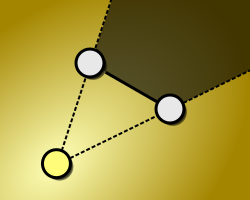
\includegraphics[width=\columnwidth]{img/light.pdf}

Imagine the robot is acting as a lamp on the board. If it sends off rays of
light, only the ones intersecting with walls, or lines, are stopped, and all
other rays continue traveling infinitely.

\subsubsection{Reverse Ray-Tracing and Line of Sight}

Let's have each node on the board draw a line segment to the current node on the
board. From there, we can check to see if this line segment drawn intersects any
polygons on the board. If it does, then we can conclude that the node is not
directly visible or accessible.

\subsubsection{Optimizations}

Performance wasn't an important goal for our system, but if you need more speed
from your system, these a few notes can be of use when optimizing.

\begin{itemize}
    \item Visibility is mutual, meaning that if one point is visible from the
          other, the opposite must be true.
    \item If a board is statically laid out, visibility never changes, an so
          such results can be cached.
\end{itemize}

\subsection{Dijkstra's Algorithm}

Dijkstra's Algorithm is an extremely popular algorithm, excellent for deducing
perfectly optimal paths in a variety of situations, and for it's design, it has
been proven mathematically optimal in terms of performance, executing in
\(\mathrm{O}\!\left(n^2\right)\) time, where \(n\) is the number of vertices, or
nodes. It has been used for both the obvious, such as in navigation systems, to
the not-so-obvious, such as phone-call routing.

Dijkstra's Algorithm works to reduce the ``cost'' of travel. For simplicity
sake, we only count the cost of translational movement, which parallels the
distance the robot travels. It's quite possible, and trivial, to modify the
algorithm to factor in the ``cost'' of rotational movements and the like.
However, For our example, whenever we say cost, read the distance to travel. As
Dijkstra's algorithm works in a purely relational manner, the units used don't
matter.

\subsubsection{Pseudo-code}

\begin{enumerate}
    \item Make a dictionary\footnote{A dictionary, or a hash-map or hash-table
          is a data structure that relates one piece of data to another.
          Thinking of it in terms of an actual dictionary, you relate the key,
          the word, with the value, the definition.} relating each node to the
          current shortest path to that point. For each node, let the beginning
          undefined path equal infinity\footnote{If this isn't possible or
          easy in your environment, assign it some special constant, such as
          \texttt{null} or Python's \texttt{None}, and note that special value
          for later on, as I did in my Python reference implementation. Work
          your later numerical checks around this.}, with the exception of the
          starting node, which you should set the cost of navigation to as zero
          (Ending where you start takes no time, and thus ``costs'' nothing).
    \item Make a queue\footnote{For our purposes, this can simply be an array,
          list, or set of some sort.} of all the nodes on the graph, excluding
          the starting one.
    \item Let the current node be the starting node.
    \item For each node in the queue, calculate the cost of the path through the
          current node to that node. If this new cost is less than the previous
          least-cost path to that node, replace it in that dictionary you made.
    \item Select the lowest cost path (where the node is in the queue). This is
          an optimal path. If this path is to the end-node, you can stop. If all
          the nodes have infinite cost, and you have not generated a path to the
          end-node yet, there is no possible path.
    \item Remove the final node from this least-cost path from the queue, and
          make it the new current node. Jump back to step 4.
\end{enumerate}

\subsubsection{An Example}

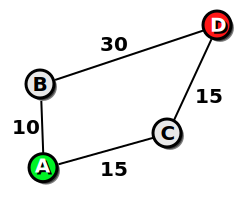
\includegraphics[width=\columnwidth]{img/dijksra.pdf}

\newcommand{\pydict}[1]{\texttt{\{#1\}}}
\newcommand{\pylist}[1]{\texttt{[#1]}}
\newcommand{\pyinf}{\(\mathtt{\infty}\)}

Following the above diagram and described algorithm, we can trace the execution
of such. Data structures will be shown in a Python manner. Specifically, the
dictionary will be expressed in the form \pydict{key=value}, and the list/queue
will be expressed as \pylist{a, b, c}.

\begin{enumerate}
    \item Our dictionary starts as \pydict{a=0, b=\pyinf, c=\pyinf, d=\pyinf}.
    \item Our queue starts as \pylist{b, c, d}.
    \item Our current node starts as a.
    \item The only directly accessible nodes from node A are B and C, each with
          a cost of 10 and 15 units respectively. Our dictionary becomes
          \pydict{a=0, b=10, c=15, d=\pyinf}
    \item Our least-cost path from the queue is through node B.
    \item Our queue becomes \pylist{c, d} as our current node becomes node B.
    \item The only directly accessible node from node B that hasn't already been
          visited (is still in our queue) is node D. The cost to get to node D
          through node B is 40 units. 40 units is less than \pyinf, so our
          dictionary becomes \pydict{a=0, b=10, c=15, d=40}.
    \item Our least-cost path from the queue is through node C.
    \item Our queue becomes \pylist{d} as our current node becomes node C.
    \item The only directly accessible node from node C that hasn't already been
          visited is node D. The cost to get to node D through node C is 30
          units. 30 units is less than 40 units, so our dictionary becomes
          \pydict{a=0, b=10, c=15, d=30}.
    \item We now have our optimal path to node D, our end-node, in the form of
          \(\mathrm{a}\to\mathrm{c}\to\mathrm{d}\).
\end{enumerate}

\section{Existing Problems}

\subsection{Working With a Radius}

Up this point, we've treated our robot as in infinitely small entity.
Unfortunately for us, the vast majority of robots have a non-zero volume. A
simple way of doing this is to outset each polygon that composes the board a
distance equal to the radius of the robot, and to work with that outset version.
There are several general ways of doing this.

\subsubsection{Constant Distance}

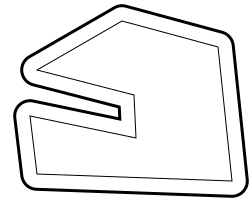
\includegraphics[width=\columnwidth]{img/complex_outset.pdf}

The most accurate way to outset a polygon is to draw a new shape around the
polygon, ensuring a constant distance. Unfortunately, the behaviors of this
system can be somewhat complex, as seen in the example diagram. Outward-facing
vertices form arcs, and so the end result is not a polygon. If one wanted to
simulate this system, they could form approximations of these curved areas by
circumscribing polygons around them.

\subsubsection{Shifting the Edges}

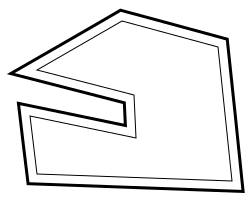
\includegraphics[width=\columnwidth]{img/simple_outset.pdf}

A much simpler approach, is to simply outset the edges, forming new lines, and
then to connect them. The na\"ive algorithm used in our sample implementation to
expand each polygon is as follows:

\begin{enumerate}

    \item For each line segment, find it the slope of a line perpendicular to it
          (find the negative inverse, \(-\frac{\Delta x}{\Delta y}\)).
    \item Find a point on the original line segment.
    \item Using the point and perpendicular slope, derive a line segment
          extending from a (any) point on the original line segment outward
          \footnote{You can easily determine what way is outward if the
          polygon's points are in a known order, such as clockwise or
          counter-clockwise}, with a length equal to the desired outset
          distance.
    \item Take the second point of the newly formed line-segment. Form an
          infinitely extending line that passes through that second point with
          the slope of the original line segment (a parallel line).
    \item Once you have these parallel lines for each edge of the base polygon,
          find the intersection points\footnote{To do this, think back to
          algebra, where you set one equation equal to the other and solved} for
          the lines corresponding to consecutive edges on the base polygon. The
          new polygon can be formed from these intersection points.

\end{enumerate}

A few special handlers should be added to deal with horizontal and vertical
lines. Many languages include support for \(-0\) and \(\pm\inf\) in their
floating-point implementations, and these may be of use.

\noindent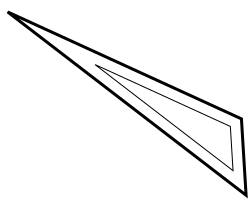
\includegraphics[width=\columnwidth]{img/simple_outset_acute.pdf}

The disadvantage of such an approach can be seen when one is working with very
acute angles. Fortunately for us, most board layouts consist of little more than
right angles, and with right and obtuse angles, such a disadvantageous effect is
minimized.

\subsection{Edge Cases}

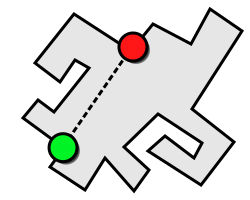
\includegraphics[width=\columnwidth]{img/line_of_sight_flaw.pdf}

Our line-of-sight algorithm works for the majority of cases. However, when first
conceived, an ``edge''-case was ignored. If the point of perspective and the
viewed point are both points on the same polygon, it is possible that a our
line-of-sight algorithm would fail to catch that the points are not visible.

Simply saying that if two nodes are on the same polygon they are not visible
from one another would be an inaccurate statement, so a more intricate solution
to the conundrum had to be found.

The system that we ended up using was a rather blunt one.

\subsubsection{Polygon Triangulation}

Polygon triangulation refers to a common practice in graphics programming by
which one takes an arbitrary polygon, convex\footnote{A polygon that only has
outward facing vertices, an example being any \textit{regular} polygon.} or
concave \footnote{A polygon that ``caves'' in upon itself.}, and turns it into a
set of triangles. This is done simply because triangles tend to be easier to
work with, as far more assumptions can be made about them.

There are a variety of ways of performing such a task, some easy, some complex.
Rather than implementing our own system, we managed to procure a piece of Java
code to do the task, and we ported the system over to Python.

The Java code was donated under public domain to the project by \texttt{asarkar}
on the \texttt{\#xkcd-cs} irc channel on \texttt{irc.foonetic.net}. (Thanks,
\texttt{asarkar}!)

\subsubsection{Applying Triangulation to Line-of-Sight}

On top of our prior checks, our system does the following for each polygon on
the map:

\begin{enumerate}
    \item Triangulate the polygon.
    \item Perform additional intersection checks with the lines formed by
          triangulation. If there is an intersection, the nodes are not visible.
    \item Check to see if our line is the same as one of the lines formed by the
          triangulation. If so, the nodes are not visible from one another.
\end{enumerate}

\section{Conclusion}

\subsection{Reference Implementation}

Our reference implementation is written in Python, or more specifically, in an
implicitly statically typed subset of the language, known as RPython. The code
has been specially crafted to run under Jython 2.5 and up, CPython 2.5 and up,
and CPython 3.1 and up\footnote{The Python 2.x and 3.x series are not entirely
compatible however they share many similarities, such that if one is careful,
they can support both with the same code-base. Python 3.x is meant to replace
the 2.x series, but both are currently supported by the Python Software
Foundation, and both are in common use.}. Other versions and implementations
should work, but simply have not been tested.

The implicitly static nature of the design, and the use but lack of dependence
of on Object-Oriented Programming should make porting to other languages such as
Java and C trivial. The end implementation, despite it's complexity, is short
(less than 1000 lines of code).

The code is available on Github under the GNU GPLv3 at
\url{https://github.com/CBCJVM/python-pathfinding}.

\subsection{Closing Thoughts}

The entire system was designed in a modular form. If nothing else, this paper
demonstrates the powers of encapsulation and subdivision. While each algorithm
is not perfect performance-wise, they work well enough for the desired purpose,
and more importantly, a superior algorithm could easily be dropped in as a
replacement, thanks to the modular design.

As a more personal message, opening this technology to the community should
hopefully provide small struggling teams with a powerful tool, and make next
year's robots all the more interesting.

Keep Hacking!

\section{Works Cited}

\printbibliography[heading=blank]

\end{multicols}

\vfill

\begin{footnotesize}
    This paper can be found online along with it's editing history and it's
    \LaTeX \ and \texttt{SVG} sources at
    \url{https://github.com/CBCJVM/GCER-Pathfinding-Paper-2011} (See the
    downloads button for a \texttt{PDF} version). This paper has been made
    available under the terms of the GNU Free Documentation License. Licensing
    information is available at the above link.
\end{footnotesize}

\end{document}
